\chapter{Design}

\section{Systemarkitektur}
En lille indledende tekst om hele systemet!!! Hvad er formålet med Design-afsnittet! Hvordan vil vi i afsnittet beskrive systemet (via diagrammer). 

\section{Hardware arkitektur}
Kort indledning 

\begin{figure}[H]
	\centering
	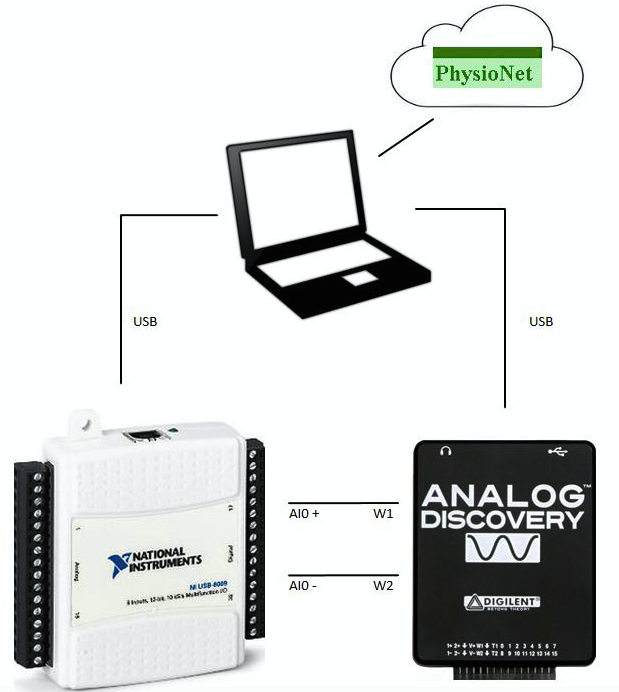
\includegraphics[width=0.8\textwidth]{Figurer/Snip20150427_1}
	\caption{Grafisk illustration af hardware opsætning}
\end{figure}

\subsection{Græseflader}
Grænseflader af forbindelserne imellem de forskellige dele af hardwaren. 

\begin{table}[H] 
	\begin{tabularx}{\textwidth}{l l X}
    \toprule
     \textbf{Forbindelse}   & \textbf{Signaltype} & \textbf{Funktionalitet}    \\ \midrule
     DAQ - Computer         & Digital & DAQ'en konverterer det analoge signal til digitalt og videresender det til 							  computeren. Informationen sendes begge veje. \\ 
     					      \addlinespace[2mm]                                                                                                                                                                            
     Computer - Analog Discovery			& Digital & Computeren simulerer et EKG-signal og sender det til Analog Discovery.\\ 
     				    	  \addlinespace[2mm]   				                                                                                                                                                                           
     Analog Discovery - DAQ			   	& Analog & Analog Discovery	 konverterer signalet fra digitalt til analogt og videresender det til 							      DAQ'en.\\  				      
    \bottomrule                                                                                                                   
    \end{tabularx}
    \caption {Beskrivelse af grænseflader.}
    \label{tab:graenseflader}
\end{table}



\section{Software arkitektur}
Kort indledning

\subsection{GUI}

\subsection{UML klassediagram}

\subsection{Appliktationsmodel}
Applikationsmodel vil i almindelig forstand indeholde en overordnet domænemodel, herefter klassediagram samt sekvensdiagram og tilsidst et opdateret klassediagram, hvor metoderne fra sekvensdiagram er inkluderet. 

Applikationsmodellen for dette projekt består af en overordnet domænemodel, herefter sekvensdiagram for de forskellige Use Cases med tilhørende opdateret klassediagram, som beskriver metodekald og kommunikation mellem klasserne. Klassediagrammerne er undladt, da de er irrevalt for dokumentationen for projektet. Applikationsmodellen er udarbejdet udfra Use Cases, hvilket medfører at metoderne er fiktive, altså ikke hentet direkte fra softwaren.  

\subsubsection{Domænemodel}
Domænemodellen er skabt på baggrund af de fem Use Cases. Gennem navneordanalyse af Use Casene er de konceptuelle klasser fundet. I modellen beskrives, hvordan de konceptuelle klasser interagerer med hinanden. Controlleren er ikke en konceptuelle klasse, men er den, der sørger for at systemet fungerer optimalt.
\\
Der er ingen multiplicity indsat i modellen, da der kun arbejdes med et scenarie af gangen. !!!!!!!!!!!!!!!!!!!!!!!!!!!!!!!! spørg Lars 

\begin{figure}[H]
	\centering
	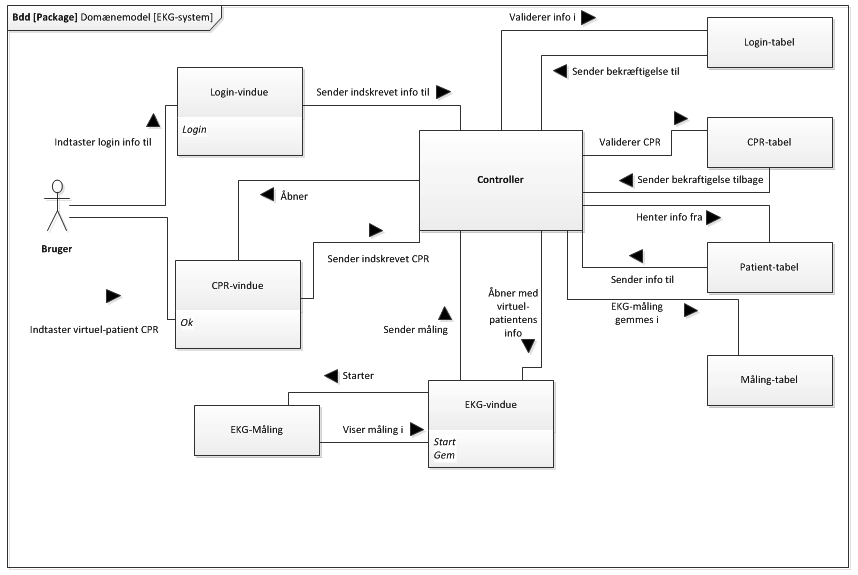
\includegraphics[width=1\textwidth]{Figurer/Snip20150429_37}
	\caption{Domænemodel af EKG-systemet}
\end{figure}

\subsubsection{Sekvensdiagram}
Sekvensdiagrammerne beskriver step-by-step via fiktive metoder forløbet i de forskellige Use Cases. Der er lavet et sekvensdiagram for hver Use Cases for at gøre systemet mere overskueligt. Et sekvensdiagram består af boundary-klasser og domain-klasser fra domænemodellen, samt en controller-klasse, som har navn efter den specifikke Use Case.  

\begin{figure}[H]
	\centering
	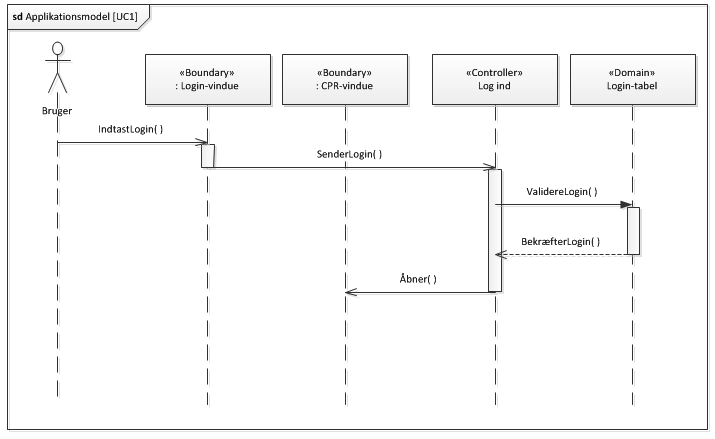
\includegraphics[width=1\textwidth]{Figurer/Snip20150429_34}
	\caption{Sekvensdiagram for UC1}
\end{figure}

\begin{figure}[H]
	\centering
	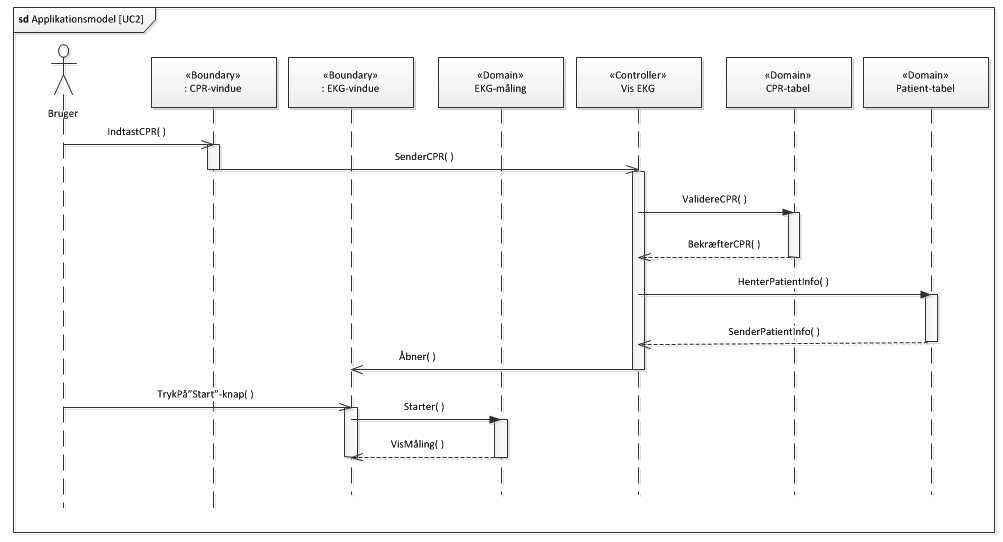
\includegraphics[width=1\textwidth]{Figurer/Snip20150429_33}
	\caption{Sekvensdiagram for UC2}
\end{figure}

\begin{figure}[H]
	\centering
	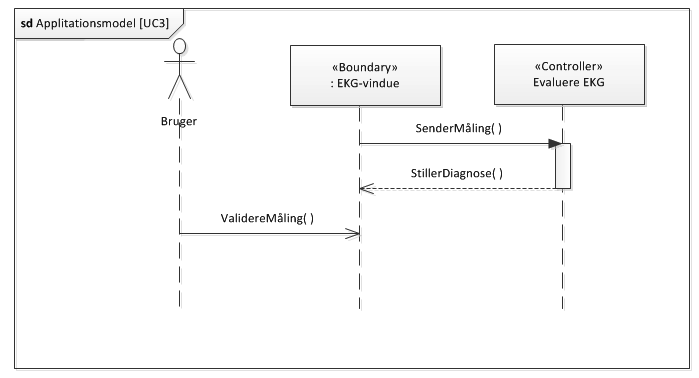
\includegraphics[width=1\textwidth]{Figurer/Snip20150429_31}
	\caption{Sekvensdiagram for UC3}
\end{figure}

\begin{figure}[H]
	\centering
	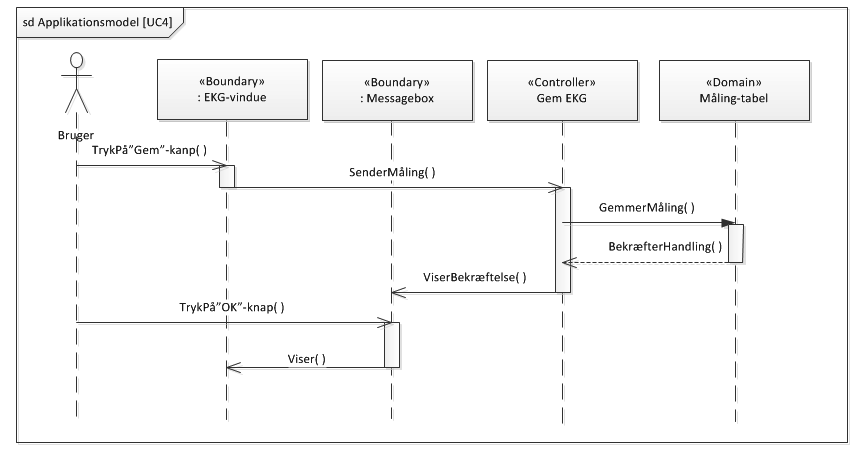
\includegraphics[width=1\textwidth]{Figurer/Snip20150429_28}
	\caption{Sekvensdiagram for UC4}
\end{figure}

\begin{figure}[H]
	\centering
	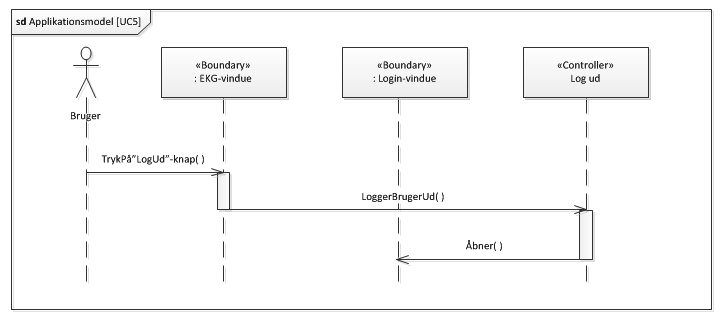
\includegraphics[width=1\textwidth]{Figurer/Snip20150429_30}
	\caption{Sekvensdiagram for UC5}
\end{figure}

\subsubsection{Opdateret Klassediagram}
De opdateret klassediagrammer indeholder metoderne fra de dertilhørende  sekvensdiagrammer - dette giver et overblik over, hvilke metoder de forskellige klasser består af.

\begin{figure}[H]
	\centering
	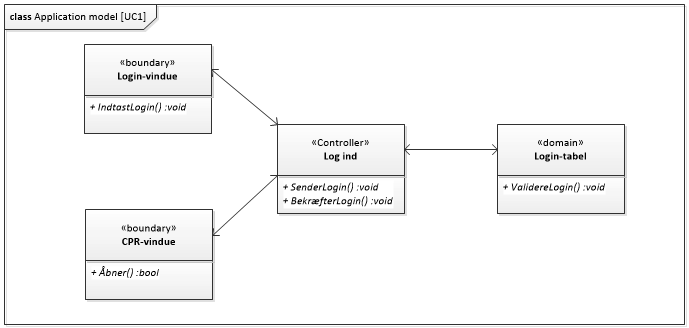
\includegraphics[width=1\textwidth]{Figurer/Snip20150429_20}
	\caption{Klassediagram for UC1}
\end{figure}  

\begin{figure}[H]
	\centering
	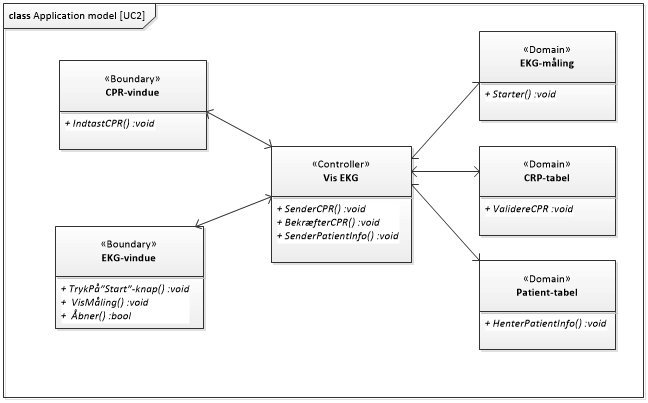
\includegraphics[width=1\textwidth]{Figurer/Snip20150429_22}
	\caption{Klassediagram for UC2}
\end{figure}

\begin{figure}[H]
	\centering
	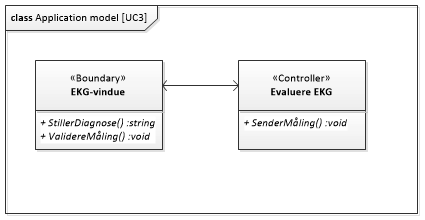
\includegraphics[width=1\textwidth]{Figurer/Snip20150429_23}
	\caption{Klassediagram for UC3}
\end{figure}

\begin{figure}[H]
	\centering
	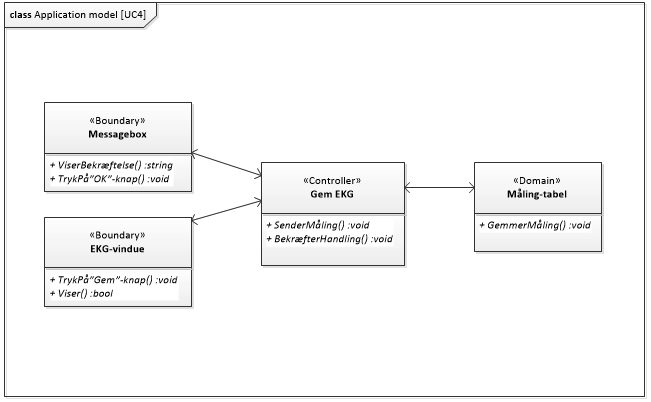
\includegraphics[width=1\textwidth]{Figurer/Snip20150429_26}
	\caption{Klassediagram for UC4}
\end{figure}

\begin{figure}[H]
	\centering
	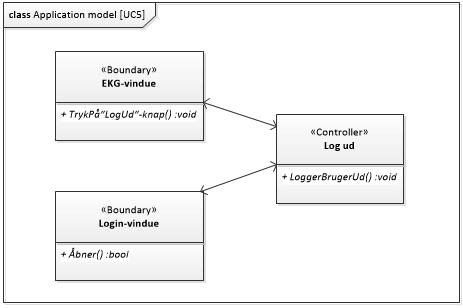
\includegraphics[width=1\textwidth]{Figurer/Snip20150429_25}
	\caption{Klassediagram for UC5}
\end{figure}





